\documentclass[a4paper]{article}
\usepackage{subfigure}
\usepackage{wrapfig}
\usepackage{caption}
\usepackage{color}
\usepackage{url}
\usepackage{amsthm}
\usepackage{amsmath}
\usepackage[utf8]{inputenc} % čudni karakteri
\usepackage{graphicx}
\usepackage[english, serbian]{babel}
\usepackage[unicode]{hyperref}
\hypersetup{colorlinks,citecolor=green,filecolor=green,linkcolor=blue,urlcolor=blue}

\newtheorem{primer}{Primer}[section]
\newtheorem{teorema}{Teorema}

\begin{document}

\title{Obrazovanje u Srbiji\\ \small{Seminarski rad u okviru kursa\\Tehničko i naučno pisanje\\ Matematički fakultet}}

\author{Jovana Tasovac\\ j.tasovac2003@gmail.com \and Marina Vračarić\\ marina.vracaric03@gmail.com \and Filip Mančić \\ mancicff@gmail.com \and Anastasija Mandić \\ anastasija.mandic2003@gmail.com}
\date{15.~novembar 2022.}
\maketitle
\abstract{
U ovom radu je ukratko predstavljeno obrazovanje u Srbiji kroz istoriju, od samih začetaka pa sve do onlajn obrazovanja  koje je bilo jedina mogućnost za vreme pandemije. Takođe, prikazano je obrazovanje u Srbiji u odnosu na ostale države, kao i prednosti i mane školovanja u istoj.
\emph {Ključne reči:} obrazovanje, Srbija, stanovništvo, nastava, škola
}
\tableofcontents

\newpage

\section{Uvod i istorijat}
\label{sec:uvod}

\vspace{0.4cm}
Prvi začeci obrazovanja u Srbiji vuku svoje korene još iz srednjeg veka. Tadašnja srpska država je raspolagala određenim obrazovnim sistemom. Glavni rasadnici pismenosti i školovanja jesu bili manastiri, a procvat samog obrazovanja Srbija je doživela za vreme dejstvovanja Svetog Save. Kako je obrazovanje postajalo sve učestalije, otvorile su se prve škole, dok su se takođe na srpskom dvoru i u kućama velikih vlastelina deca učila raznim veštinama: pisanju, čitanju, ukrašavanju, tkanju, trgovini, zanatima…sve do borilačkih veština.\\
U nešto kasnijem periodu, padom Srbije pod tursko ropstvo, čitav napredak nad srpskim obrazovanjem je progresivno bivao gašen, Turci su nametali narodu njihovu kulturu i veru i na taj nacin uništavali srpski narod. Čak i dan danas postoji pregršt reči u srpskom rečniku koje su turskog porekla, što samo dokazuje koliki su uticaj imali na srpski narod.
 Nakon tog teškog perioda za Srbiju, usledili su neki bitni događaji sto se srpskog obrazovanja tiče:
 \begin{itemize}
    \item  U Beogradu je između 1718. i 1739. postojala Mala srpska škola, danas poznata kao osnovna škola "Kralj Petar I""\cite{referenca1}
    \item Početkom 18. veka, u porti crkve Svetog Đorđa, 1703. god. osnovana je prva škola u Petrovaradinskom Šancu (današnjem Novom Sadu) - Srpska pravoslavna osnovna škola
    \item 1791. godine je u Sremskim Karlovcima osnovana Karlovačka gimnazija\cite{referenca2}
    \item Tokom Prvog srpskog ustanka, u Beogradu je 1808. osnovana Velika škola zaslugom Ivana Jugovića i Dositeja Obradovića
    \item U Kragujevcu je oktobra 1838. osnovan Liceum Knjažestva serbskog, prva viša škola u Srbiji. On je 1841. premešten u Beograd. Licej je postojao do 1863. kada prerasta u Veliku školu, koja je imala tri fakulteta: Filozofski, Tehnički i Pravni.\cite{referenca3}
\end{itemize}
Dolazimo do perioda 20. veka – ovaj vek obeležava osnivanje Beogradskog univerziteta\cite{referenca4} 1905. godine. Posle Drugog svetskog rata iz Beogradskog univerziteta su se izdvojili Univerzitet u Novom Sadu (1960), Nišu (1965), Prištini (1970), Podgorici (1974) i Kragujevcu (1976).\cite{referenca4}
U narednom veku obrazovanje se razvijalo jako brzo, škole su postale sastavni deo dana obrazovanja svakog deteta do 2020. godine, gde se sistem rada privremeno menja.




\section{Onlajn nastava}
\label{sec:Onlajn}
Nakon proglašenja pandemije korona virusa, većina nacija zatečena istom je odlučila da svoju edukaciju premesti na novu platformu i oproba u novom sistemu učenja – onlajn nastava. Nedostatak vremena u svakodnevnom životu i pre pandemije, ali i želja za novim znanjem i drugačijim načinom obrazovanja, podigli su onlajn nastavu na višu lestvicu. Iz tih razloga, većina edukativnog sadržaja se može pratiti iz udobnosti toplog doma što je ujedno i najveća prednost ovakvog načina edukacije. U trenutku pojave pandemije, sistem onlajn nastave definitivno nije bio dovoljno razvijen da bi se moglo reći da nije dolazilo do gubitaka u znanju. Ono što je predstavljalo najveći problem jeste loša organizacija, nedostatak kompjuterske pismenosti i prebrza tranzicija na takav sistem. Kvalitet ovog oblika nastave ne zavisi od karakteristika istog, već od sposobnosti nastavnika i učenika da je primenjuju. Internet, kao prostor na kome se realizuje onlajn nastava, nam nudi mogućnost da realizujemo sve ove oblike rada, a na nama je da biramo šta želimo. Ali, da bismo odabrali da realizujemo neki oblik ili metodu, moramo da znamo određene veb-alate i softvere za rad u ovom prostoru. 

Početak onlajn nastave definitivno su obeležili časovi emitovani preko televizije(slika \ref{fig:onlajn nastava}). Naizgled zanimljiv i koristan format, jer na neki način stvara obavezu zbog emitovanja nastave u određeno vreme, što dovodi do zaključka da nema mesta propuštanju nastave. Ali na drugi pogled, po ovom sistemu rada učenici ovde ulažu najmanje energije, pa samim tim toliko znanja i dobiju. Da je kvalitet samih predavanja bio dobar – to je činjenica, ali kvalitet samog sistema učenja je jako osporiv. Ovo ne predstavlja kvalitetnu onlajn nastavu.\cite{referenca5}

\begin{figure}[h!]
        \centering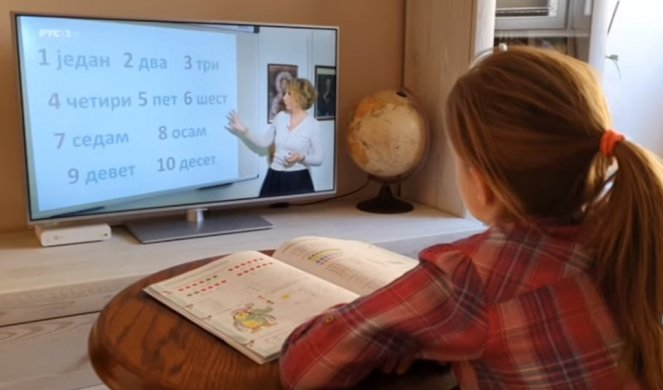
\includegraphics[height=3cm]{onlajn-nastava.jpg} 
        \caption{}
        \label{fig:onlajn nastava}
\end{figure}
Vremenom se nastava prebacila na internet platforme za učenje poput Google Classroom-a, kombinovanim sa alatkama za prenos uživo – Google Zoom, Meet i slično. Ako isključivo radimo na ovaj način, nismo ništa promenili u odnosu na klasično predavanje u učionici. Samo prostor, odnosno nismo više u fizičkoj učionici, sada smo na internetu. Ako je učenicima bilo teško da slušaju nastavu u učionici 45 minuta, bilo bi nelogično pomisliti da bi ovakav način bio uspešniji. Sada će im biti još teže, jer nisu u školskom prostoru koji je kreiran za učenje, nego su u svojim domovima, gde imaju puno ometača, i u prostoru koji je za spavanje i zabavu. Druga negativna strana ovog vida učenja su spoljni faktori na koje se teško ili skoro uopšte ne može uticati. Samo neki od tih faktora su internet konekcija, nedostatak kamera i mikrofona, kao i nemogućnost posedovanja uređaja koji su dovoljno dobri za ovakvu nastavu (star i nedovoljno dobar hardver – nije svako u mogućnosti da priušti dobar kompjuter, laptop ili telefon, uključujući i roditelje i nastavnike).

Čak su i izvori za učenje postali onlajn – đaci za vreme takve nastave u većini slučajeva nisu morali da se trude da pišu, vec su dobijali okačene snimke predavanja, tekstualne fajlove ili PDF dokumente spremne, rezimirane, i servirane da što pre i što lakše nauče gradivo kako bi dobili što više ocena. Razlog tome su gore navedeni problemi -  često su i nastavnici želeli da olakšaju sebi muke koje donosi onlajn nastava, što je validno, ali samim tim se dokazuje da ni ovaj vid učenja nije dovoljno kvalitetan. 

Kvalitetna onlajn nastava bi predstavljala kombinaciju sve gore navedenog, plus mnogo dodatnih onlajn resursa koje sada mnogo lakše možemo iskoristiti nego u učionici. Onlajn nastava se ne može zamisliti kao kopija ili klon nastave u učionici. Nije izvodljivo. Može se pokušati, ali ono što će biti produkt toga nije kvalitetna nastava. Onlajn nastava ne treba da se zamisli kao nastava sa strukturom časova od 30 ili 45 minuta, vec treba da koristi pune mogućnosti i interaktivnost interneta čime se ispunjava pun potencijal ovakvog ucenja – interaktivne slike, prezentacije, kvizovi, igrice, ... - to su samo neki od dodatnih resursa kojima se može koristiti. Onlajn nastava mora biti koncipirana kao projektna nastava\footnote{\href{https://en.wikipedia.org/wiki/Project-based_learning}{projektna nastava} }, a idealno bi bilo kao multidisciplinarna projektna nastava\footnote{\href{https://careercenter.utsa.edu/blog/2018/05/03/multidisciplinary-studies-so-what-does-that-mean/}{multidisciplinarna projektna nastava} }. 

Nažalost, za Srbiju ne postoji nijedna zvanična statistika, ali je vredno napomenuti da su ovakvim vidom učenja druge države generalno zadovoljne. Od 2020. godine, 98\% obrazovnih ustanova u Sjedinjenim Američkim Državama je implementiralo i normalizovalo ovo kao redovan (opcionalan) način učenja.\cite{referenca6}

\section{Prednosti i mane obrazovanja u Srbiji}
\label{sec:Prednosti}

Teško je pričati o prednostima i manama obrazovanja i biti objektivan. Međutim, postoje stvari na koje definitivno treba više obratiti pažnju. Neosporivo je da Srbija često kasni u odnosu na razvijenije evropske zemlje, kao i velike zemlje drugih kontinenata,  tako da će se sistem obrazovanja neminovno razvijati u budućnosti, a o nekim problemima jednostavno treba više govoriti. Samim tim što smo generalno više konzervativna nego liberalna država, roditelji se neretko drže zastarelih stavova o tome kako decu treba terati da uče, što predstavlja koren mnogih problema u samom obrazovanju. Druge razvijenije zemlje su uveliko pokrenule roditeljske škole koje edukuju roditelje na tu temu, i o tome bi trebalo češće govoriti i normalizovati roditeljsku edukaciju kao takvu. 
U daljem tekstu će konkretnije biti predstavljene prednosti i mane obrazovanja u Srbiji.


\textbf{ Prednosti obrazovanja:}
\begin{enumerate}
    \item \textbf{Zastupljenost obrazovnih ustanova}
    \\Veliki gradovi u Srbiji poseduju ustanove koje su potrebne za sve stepene obrazovanja deteta, od osnovne škole pa sve do više škole i fakulteta. Pored toga, svi manji gradovi imaju barem po jednu osnovnu i srednju školu, i uglavnom i fakultet. Vrtići, kao početak obrazovanja u životu svakog deteta, prisutni su u svakom mestu, kako državni, tako i privatni.
    \item \textbf{Bezbednost u školama}
    \\Bezbednost u našim školama i obrazovnim ustanovama je na visokom nivou. Svaka škola ima svog policajca ili čuvara koji je zadužen da u svakom trenutku pazi na bezbednost dece. Na taj način, maksimalno je smanjen broj pojavljivanja nepoželjnih osoba u okolini, kao i u samim ustanovama.
     \item \textbf{Raznovrsnost fakulteta}
     \\Nakon završenog srednjeg obrazovanja, veliki broj učenika ima poteškoća sa odabirom daljeg školovanja. Međutim, ogroman spektar različitih mogućnosti kako fakulteta, tako i viših škola, olakšava im te muke, i dozvoljava svakom pojedincu da pronađe sebe i svoju budućnost.
     \item \textbf{Način predavanja}
     \\Iako način predavanja i pristup profesora ovde igra veliku ulogu, možemo se složiti da je način predavanja  svuda relativno sličan. Konstantne provere znanja uče decu kako bolje da organizuju svoje vreme i prave im radne navike koje će im u budućnosti biti prekopotrebne. Takođe, česta usmena ispitivanja  grade njihovu sposobnost komunikacije i boljeg izražavanja misli. \cite{referenca7}

\end{enumerate}

\textbf{ Mane obrazovanja:}
\begin{enumerate}
    \item \textbf{Bezbednost}
     \\Iako su deca bezbedna od ljudi sa strane, to se ne može reći i za bezbednost unutar škole. U poslednje vreme ogroman problem u nižim stepenima obrazovanja (osnovno i srednje) predstavlja vršnjačko nasilje. Kako psihičko, tako i fizičko pravi veliki problem nastavnicima i roditeljima. U poslednjih par godina, sa porastom uticaja društvenih mreža u velikoj meri je poraslo takozvano internet nasilje (cyberbullying). Deca se kriju iza lažnih profila i vređaju jedni druge po rasnim, verskim i materijalnim osnovama. Na ovom problemu se intenzivno radi, ali je njegovo iskorenivanje vrlo teško. 
     \item \textbf{Ocenjivanje učenika}
     \\Ocenjivanje u Srbiji svodi se na pet ocena. To je veoma mali prostor da bi se prikazale finese u znanju. Roditelji ga smatraju prilično grubim i vrlo često nerealnim pokazateljem znanja. Takođe, često se događa da učenik bude oštećen ocenom što može da se odrazi na njegovo mentalno zdravlje - o tome čak i svedoči da se ocene pri unosu u eDnevnik ne prikazuju prvih 48h iz psiholoških razloga.
     Što se tiče fakulteta, ocenjivanje samo jednom u semestru, i to svih predmeta od jednom, stvara ogroman stres studentu, i zbog toga nekad njegovi rezulati nisu plod njegovog rada već posledice stresa. Međutim ovaj problem je rešen na većini fakulteta u Srbiji u proteklih par godina uvođenjem Bolonjskog sistema \footnote{\href{https://www.eduinfo.ba/zakoni-u-obrazovanju}{Bolonjski sistem} }.

\end{enumerate}
\section{Srbija u poređenju sa ostatkom sveta}

Veliki broj ljudi smatra zemlje istočne Azije, to jest Kinu, Japan i Hong Kong, državama sa najboljim obrazovnim sistemom na svetu. Prva razlika nastaje još pre nego što deca krenu u školu, odnosno, stanovnici ovih država se trude da svojoj deci već od malih nogu stvaraju radne navike i uče ih da im slobodno vreme i zabava budu edukativnog tipa. Mnogo ranije se deca upoznaju sa čitanjem, pisanjem, i generalno naukom i umetnošću. Sistem u Aziji je takav da su deca u školi veliki deo dana, dok im ostatak dana zauzima rađenje domaćih zadataka. Čak i ako nađu još neko slobodno vreme, uglavnom ga usmeravaju ka vannastavnim aktivnostima kao što su sviranje nekog instrumenta, učenje stranog jezika i slično.\\
Postavlja se pitanje:\\ \textbf{Koje države imaju najobrazovanije stanovnike na svetu?}\\
Na ovo pitanje nije tako lako dati odgovor kao što bi prvo ljudi pomislili, jer je "najobrazovaniji" neprecizan termin. Na primer, koja bi se smatrala obrazovanijom: zemlja u kojoj je 50\% stanovnika završilo srednje obrazovanje, a 25\% steklo visoko obrazovanje, ili zemlja u kojoj je 100\% stanovnika završilo srednje obrazovanje, ali ni jedan nema diplomu fakulteta?
Uprkos neodređenosti pojma, višestruka istraživanja i studije dale su sve od sebe da utvrde koje zemlje imaju najobrazovanije stanovništvo. Jedna od najcenjenijih analiza dolazi od Organizacije za ekonomsku saradnju i razvoj(Organization for Economic Cooperation and Development), koja je objavila svoju listu najobrazovanijih zemalja sveta 2018. U tabeli  \ref{tab:tabela1} je data lista najobrazovanijih 10 država po njihovom istraživanju.\cite{referenca8}

\begin{table}[h!]
\begin{center}
\caption{Top 10 najobrazovanijih država(2018)}
\begin{tabular}{|c|l|} \hline
\textbf{država}& \textbf{\% obrazovanog stanovništva}\\ \hline
Kanada &56.27\\ \hline
Japan &50.50\\ \hline
Izrael &49.90\\ \hline
Južna Koreja &46.86\\ \hline
Velika Britanija &45.96\\ \hline
SAD &45.67\\ \hline
Australija &43.74\\ \hline
Finska &43.60\\ \hline
Norveška &43.02\\ \hline
Luksemburg &42.86\\ \hline
\end{tabular}
\label{tab:tabela1}
\end{center}
\end{table}

Sa druge strane sistem u Srbiji je takav da su deca na početku u školi samo deo prepodneva, kako bi se adaptirala, i sa godinama se navikavala da su u školi sve duže i duže. Jasan je zaključak da zahvaljujući tolikom forsiranju radnih navika dece u Aziji, ona često izrastaju u mnogo vrednije ljude sa višim ciljevima i životnim standardima. 
 
Po nekim drugim istraživanjima, prvak u Evropi što se tiče obrazovanja jeste Estonija. Ono po čemu se ona definitivno izdvaja, bila prva ili ne, jeste da je zanimanje profesora na fakultetu, ili nastavnika u srednjim i osnovnim školama značajno cenjenije i plaćenije nego kod nas. Deca su tamo vaspitana da mnogo više poštuju profesore, koji, da bi to postali, moraju da završe vrlo teške fakultete  i budu veoma cenjeni i uspešni u svom stručnom polju. Takođe, svako dete u Estoniji ima jednaka prava na školovanje, bez obzira na poziciju i bogatstvo svojih roditelja. Svaka škola je podjednako pristupačna svima, i u koju će školu dete ići zavisi samo od njegovog truda i dobrih ocena. To se nažalost ne može reći i za školovanje u Srbiji.


Generalno se smatra da je osnovno i srednje obrazovanje u Evropi i kod nas dosta kvalitetnije od obrazovanja u Americi. Razlog tome je što kvalitet obrazovanja u Americi zavisi najviše od količine novca koje se uloži u njega. Kod nas ima dosta privatnih škola, ali je osnovno i srednje obrazovanje besplatno i pristupačno svima.

Univerzitet u Beogradu je priznat u svetu i može pružiti veoma visoko znanje svojim studentima. Iako nismo pri vrhu spiska univerziteta na celom svetu, studenti iz Srbije su često kasnije veoma cenjeni stručnjaci u svom polju.
\label{sec:Srbija}
\newpage
\section{Zaključak}
\label{sec:Zaključak}
Naš rad na ovu temu bio je inspirisan važnošću obrazovanja za svaki narod, pa tako i za naš. Srbija poseduje jak temelj školstva koji može samo da se unapredi, kako bi ostalim generacijama znanje bilo pristupačnije i proces učenja zanimljiviji. Iako nesavršen, sistem obrazovanja ove države već godinama uspeva da izvede stanovništvo na pravi put. Generalno se naši učenjaci sjajno kotiraju i po znanju i po dostignućima u inostranim zemljama. Smatramo da imamo ogroman potencijal za dalji napredak u smislu obrazovnog sistema i da je progresija u budućnosti definitivna.
\addcontentsline{toc}{section}{Literatura}
\appendix

\iffalse
\bibliography{seminarski} 
\bibliographystyle{plain}
\fi

\begin{thebibliography}{9}
\bibitem{referenca1} \emph{ Osnovna škola Kralj Petar I}\\ 
\url{https://en.wikipedia.org/wiki/King_Petar_I_Elementary_School} 5.12.2022.
\bibitem{referenca2} \emph{Karlovačka gimnazija }\\ \url{https://en.wikipedia.org/wiki/Karlovci_Gymnasium} 5.12.2022.
\bibitem{referenca3} \emph{Liceum }\\ \url{https://en.wikipedia.org/wiki/Lyceum_of_the_Principality_of_Serbia} 5.12.2022.
\bibitem{referenca4} \emph{ Istorijat}\\ \url{https://sr.wikipedia.org/sr-el/Obrazovanje_u_Srbiji} 5.12.2022.
\bibitem{referenca5} \emph{Onlajn nastava}\\ \url{https://okc.rs/sta-jeste-a-sta-nije-onlajn-nastava/} 5.12.2022.
\bibitem{referenca6} \emph{Statistika}\\ \url{https://upskillwise.com/online-learning-statistics/} 5.12.2022.
\bibitem{referenca7} \emph{Prednosti i mane }\\ \url{https://www.skolskiportal.rs/clanci/1074-prednosti-i-mane-nasih-skola} 5.12.2022.
\bibitem{referenca8} \emph{Organization for Economic Cooperation and Development }\\ \url{https://worldpopulationreview.com/country-rankings/most-educated-countries} 6.12.2022.
\end{thebibliography}

\appendix
\end{document}
